%% LaTeX2e class for student theses
%% sections/content.tex
%% 
%% Karlsruhe Institute of Technology
%% Institute for Program Structures and Data Organization
%% Chair for Software Design and Quality (SDQ)
%%
%% Dr.-Ing. Erik Burger
%% burger@kit.edu
%%
%% Version 1.3.5, 2020-06-26

\chapter{Feature generation}
\label{ch:Content1}
%% ==============

The first step of most machine learning tasks is to extract relevant features from our dataset.
In the case of out data, we can make use of the special structure of catalyst molecules when generating out features.
Since location and rotation of the molecule has no effect on it's properties, our features should not contain any information about these.

The dataset can formally be described as a set $D$. \\
$D$ represents a set of molecules. Each molecule is represented by a list of touples of (atom, location in 3d space). \\
$D = \{(m_0, m_1, \dots, m_n)| m_i \in \{ (a, l): a \in A, l \in \mathbb{R}^3\}, i = 0..n\}$ with $A = M \cup \{h\} \cup A_r$ being a set of atoms, where $M$ are all metal atoms, $h$ is a hydrogen atom, $A_r$ are all other atoms. 
Each atoms has certain properties, such as a Van-der-Waals radius. 
Since we're looking at catalysts, we can set the following conditions to our molecules $(m_0, m_1, \dots, m_n) \in D$:
\begin{itemize}
  \item $m_0 \in M \times \mathbb{R}^3$, the first atom is a metal atom.
  \item $m_1, m_2 \in (h, l), l \in \mathbb{R}^3$, the second and third atoms are hydrogen atoms.
\end{itemize}

\section{Translational invariance}


In a first step, the molecule $m=((a_0, l_0),\dots,(a_n, l_n)) \in D$ is centered around a unique point.
Since every catalyst has exactly one metal atom, the molecule can be centered around this atom.
Formally, the metal atom is set to location $(0,0,0)$ and all other atoms are translated accordingly.

$m' = m -^E l_0$ \footnote{$\circ^E$, with $\circ$ being any pairwise operator, will be used as a abbrevation for a pairwise application of $\circ$ to the location of each atom in a molecule.
\\
$x \circ^E ((a_0, l_0), (a_1, l_1), ... ,(a_n, l_n)) = ((a_0, x \circ l_0), (a_1, x \circ l_1), ... (a_n, x \circ l_n))$
\\
and
\\
$((a_0, l_0), (a_1, l_1), ... (a_n, l_n)) \circ^E x = ((a_0, l_0 \circ x), (a_1, l_1 \circ x), ... (a_n, l_n \circ x))$
}


\section{Rotational invariance}

The next step is to find a unique rotation.
This problem can be devided into 2 parts.
By definition the second and third atom of any molecule in the dataset are hydrogen atoms.
These atoms form a reaction pocket. %TODO: Describe reaction pocket somewhere
The reaction pocket will become the new top of the molecule.
Since every atom has exactly 1 reaction pocket, 2 more degrees of freedom can be removed, only allowing for rotations around the z-axis.


\subsection{Define top point}

The location of the reaction pocket $l_r$ is calculated by taking the mean of the location of the first 2 hydrogen atoms, so:

$l_{pocket} = \frac{l'_1 + l'_2}{2}$

The molecule is then rotated so that the reaction pocket will be straigt up from the center point, so $l_{pocket}' = (0,0,z)$.
Using a rotational matrix, all points are rotated around the center accordingly.

For finding a rotational matrix, first the angles between $l'_{pocket}$ and the z-axis $(0,0,1)$ are computed.
More specifically, the angle $\alpha$ between $(l'_{pocket}[0], l'_{pocket}[1], 0)$ and $(1,1,0)$ that needs to be rotated around the z-axis, 
the angle $\beta$ between $l'_{pocket}$ and $(1,1,1)$ that needs to be rotated around the y-axis afterwards.

$\alpha = \arccos \left(
  \frac{
  \begin{pmatrix}
    l'_{pocket}[0] &
    l'_{pocket}[1] &
    0
  \end{pmatrix}^T
  \cdot 
  \begin{pmatrix}
    1 &
    1 &
    0
  \end{pmatrix}^T}
  {
  \begin{Vmatrix}
    l'_{pocket}[0] &
    l'_{pocket}[1] &
    0
  \end{Vmatrix}
  \cdot 
  \begin{Vmatrix}
    1 &
    1 &
    0
  \end{Vmatrix}}
\right)
$

$\beta = \arccos \left(
  \frac{
    l'_{pocket}
  \cdot 
  \begin{pmatrix}
    1 &
    1 &
    1
  \end{pmatrix}^T}
  {
  \begin{Vmatrix}
    l'_{pocket}
  \end{Vmatrix}
  \cdot 
  \begin{Vmatrix}
    1 &
    1 &
    1
  \end{Vmatrix}}
\right)
$

First, the y-part of $l'_{pocket}$ is eliminated by rotating the point around the z-axis using a rotation matrix.

$
R_z =
\begin{pmatrix}
  \cos(\alpha) & \sin(\alpha) & 0 \\
  -\sin(\alpha) & \cos(\alpha) & 0 \\
  0 & 0 & 1
\end{pmatrix}
$

Afterwards, the remaining x-part of $l'_{pocket}$ is eliminated by rotating the point around the y-axis.

$
R_y =
\begin{pmatrix}
  \cos(\beta) & 0 & -\sin(\beta) \\
  0 & 1 & 0 \\
  \sin(\beta) & 0 & \cos(\beta) 
\end{pmatrix}
$

The full rotation can be described as $R = R_y \cdot R_z$

This rotation is applied to all atoms, so:

$m'' = R \cdot^E m'$


\subsection{Slice molecule}

Since the molecule can be arbitrarly rotated around the z-axis, no clear start point for the rotation around the z-axis can be defined.
To cope with that, the model is sliced along the z-axis. 
The contour is then described using a rotationally invariant contour descriptor.

\paragraph{Slicing}

Along the z-axis, starting from $z_{start}$ to $z_{end}$, the molecule is sliced in a distance of $layer_{height}$.
$z_{start}, z_{end}, layer_{height}$ are tuning parameters. 
Here, $z_{start}, z_{end}$ are chosen so that all molecules from the dataset fully fit into the boundaries.
TODO: Layer height %TODO: Why is layer height chosen as it is? 

By slicing a molecule at a location $z_{slice}$, every slice contains a subset of atoms of the current molecule with a radius at the current height.

\dots

\begin{figure} [h]
  \centering
  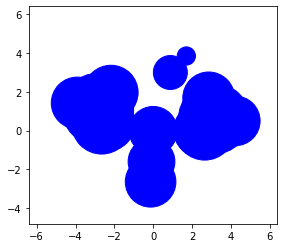
\includegraphics[width=0.5\textwidth]{figures/slice-iso.png} % for .pdf files etc use \includegraphics{test.pdf}
  \caption{A slice with isolates.}
  \label{fig:slice}
\end{figure}

\subsection{Invariant contour describition}

After slicing the molecule, a set of circles $C$ for every slice is left \autoref{fig:slice}.
These circles can be partially or fully intersecting. 

To describe the contour, a fourier contour descriptor is used.
This contour descriptor allows to easily ignore rotation of the contour and generate invariant low-dimensional features from the shape.
However, it can only work on a closed contour, so isolate islands of circles that don't intersect have to be dealt with seperately.

%TODO
TODO: Describe how the contour descriptor works

\subparagraph{Igoring isolates} 

The easiest step to get a single closed contour is to simply ignore isolate circles.
To find isoaltes, a graph is constucted. 
Each circle is node, if 2 circles intersect each other an edge is added between these nodes.
Now each connected component of the graph correlates to one closed contour. 
The component with the most nodes is the fed into the contour descriptor.

\subparagraph{Describe contour}

From the set of intersection circles, the contour needs to be extracted. 
Since the contour points need to be computed just from radius and position information, and are not rendered onto a 2D pixel grid, standard contour finding algorithms can not be used.
Instead, knoledge about the general shape is used to compute the contour. 

The contour is computed using \autoref{alg:CircleSetContour}.

First, the point "furthest to the right", so with the largest x-Value is found. 
Since the point with the highest x-Value in any circle is always at angle 0, we set the intial angle $\alpha$ and rotation vector $\vec{p}$ accordingly.
From the circle containing that point, the contour is followed from that point counter-clockwise until the first intersection with another cirlce is found \autoref{fig:contour1}.
To the list of countour sections, we add the current contour section from angle 0 to the angle of intersection.

Now, the contour of this circle is followed again until it intersects another. This is reapeated until the starting circle is reached again \autoref{fig:contour2}.

Once the starting circle is reached, the last remaing contour part of the starting circle needs to be added to the list of contour sections \autoref{fig:contour3}.

From the ordered list of contour sections, the contour points can easily be computed.
Since each contour section consits of a radius $r$, location $(x,y)$, and start- and end angle $\alpha_{start}, \alpha_{end}$, the coordinates of the contour points can simply be computed using $x_c = \cos(\alpha_c) \cdot r + x$ and  $y_c = \sin(\alpha_c) \cdot r + y$ 
for $\alpha_c = \alpha_{start} + i \cdot \Delta, \alpha_c \leq \alpha_{end}$.
$\Delta$ is a tuning paramter that specifies the resolution of the contour.

This process of going along the outside ignores all "holes" in the shape, so only the outermost contour will be part of the final result.

%\begin{theorem}
%\label{theorem:doof}
%  Wer das liest ist doof.
%\end{theorem}
%\begin{proof}
%  Weil ist so.
%\end{proof}

\begin{algorithm}[p]
\caption{\textsc{CircleSetContour}}\label{alg:CircleSetContour}


% Some settings
\DontPrintSemicolon %dontprintsemicolon
\SetFuncSty{textsc}
\SetKwFor{ForAll}{forall}{do}


% Declaration of data containers and functions
\SetKwData{Q}{Q}
\SetKwData{C}{C}
\SetKwData{G}{G}
\SetKwData{L}{L}
\SetKwData{dist}{d}
\SetKwData{pred}{pred}
\SetKwFunction{queueDeleteMin}{deleteMin}
\SetKwFunction{append}{append}
\SetKwFunction{queueInsert}{insert}
\SetKwFunction{queueDecreaseKey}{decreaseKey}
\SetKwFunction{queueContains}{contains}
\SetKwFunction{insertEdge}{addEdge}
\SetKwFunction{queueContains}{contains}
\SetKwFunction{location}{location}
\SetKwFunction{angleBt}{angle}
\SetKwFunction{angleToVec}{angleToVec}
\SetKwFunction{vecToAngle}{vecToAngle}
\SetKwFunction{intersect}{intersections}
\SetKwFunction{neigh}{neighbors}
\SetKwFunction{points}{pointsInRange}

\SetKwRepeat{Do}{do}{while}

% Algorithm interface
\KwIn{Set \C of circles}
\KwData{Graph $\G = (\C, \emptyset)$}
\KwOut{List of contour sections $\C$ in order}

% The algorithm
\BlankLine
\tcp{Generate graph}
\ForAll{$(c_1,c_2) \in \C \times \C$}{
  \If{distance$(c_1, c_2) < c_1.radius + c_2.radius$}{
    \G.\insertEdge{$c_1, c_2$}

  }
}

\BlankLine
\tcp{Find contour sections}
$c_{max} \in \{c_i \in \C | \forall m \in \{1..|\C|\}: c_m.x + c_m.radius \leqslant c_i.x + c_i.radius\}$

$c\leftarrow c_{max}$

$\vec{p} \leftarrow \begin{pmatrix}
  1 \\
  0
\end{pmatrix}$

$\alpha \leftarrow 0$

\Do{$c_{max} \neq c$}{
  \tcp{Find adjacent circle with intersection of smallest angle}
  $ \left(c_{next}, \beta \right) \leftarrow 
  \min_2{\left\{ 
    (n, \gamma)\ \middle\vert 
    \begin{array}{l}
      n \in \G.\neigh\left(c\right), \\
      \gamma  = 
        \min\left\{
          \angleBt{
            p, \intersect{n,c}
          }
        \right\}
    \end{array}
  \right\}} 
  $

  $\C.\append \left(
      \left(c , \alpha , \beta \right)
    \right)
  $

  \tcp{Calculate start direction vector of the next circle}
  $ \vec{p} \leftarrow \left( c.center + (\angleToVec(\beta) * c.radius ) - c_{next}.center\right)$
  
  $ c \leftarrow c_{next} $
  
  $  a \leftarrow \vecToAngle(\vec{p}) $

  }

  \tcp{Finish contour of last circle}
  $\C.\append \left( c_{max}, \alpha, 0 \right)$

\end{algorithm}



%\begin{figure} [bt]
%  \centering
%  \tikzstyle{node}=[circle,inner sep=0.5mm,minimum size=5.25mm,draw = black]
\tikzstyle{bright}=[fill=black!14]
\tikzstyle{dark}=[fill=black!28]
\tikzstyle{lightEdgeStyle}=[black!20]

\newcommand{\numberOfNodes}{5} % must be >= 4

\begin{tikzpicture}[scale=1.5, bend angle = 20]

% Obere Reihe
\node(Top1) at (1,1) [node, bright] {1};
\foreach \i [evaluate = \i as \lastNode using \i-1] in {2,3,...,\numberOfNodes}
{
  \node (Top\i) at (\i,1) [node, bright] {\i}
    edge[<-] (Top\lastNode);
}

% Untere Reihe
\node(Bot1) at (1,0) [node, dark] {$\infty$};
\foreach \i [evaluate = \i as \lastNode using \i-1] in {2,3,...,\numberOfNodes}
{
  \node (Bot\i) at (\i,0) [node, dark] {$\infty$}
    edge[<-, lightEdgeStyle] (Bot\lastNode);
}

% Kanten zwischen den Reihen
\foreach \i in {1,2,...,\numberOfNodes}
{
  \foreach \j in {\i,...,\numberOfNodes}
   {
     \draw[lightEdgeStyle] (Bot\i) -- (Top\j);
   }
}

% Pfeile nach rechts
\pgfmathparse{\numberOfNodes - 2}
\foreach \i [evaluate = \i as \nextNode using \i+2] in {1,2,...,\pgfmathresult}
{
 \foreach \j [count=\nodeIndex from \nextNode] in {\nextNode,...,\numberOfNodes}
 {
   \draw[->, lightEdgeStyle] (Bot\i) to [bend right] (Bot\nodeIndex);
 }
}

\end{tikzpicture} 
 % for .pdf files etc use \includegraphics{test.pdf}
%  \caption{Slice with isolate circles.}
%  \label{fig:somegraph}
%\end{figure}


\begin{figure}[!htb]
  \minipage{0.32\textwidth}
    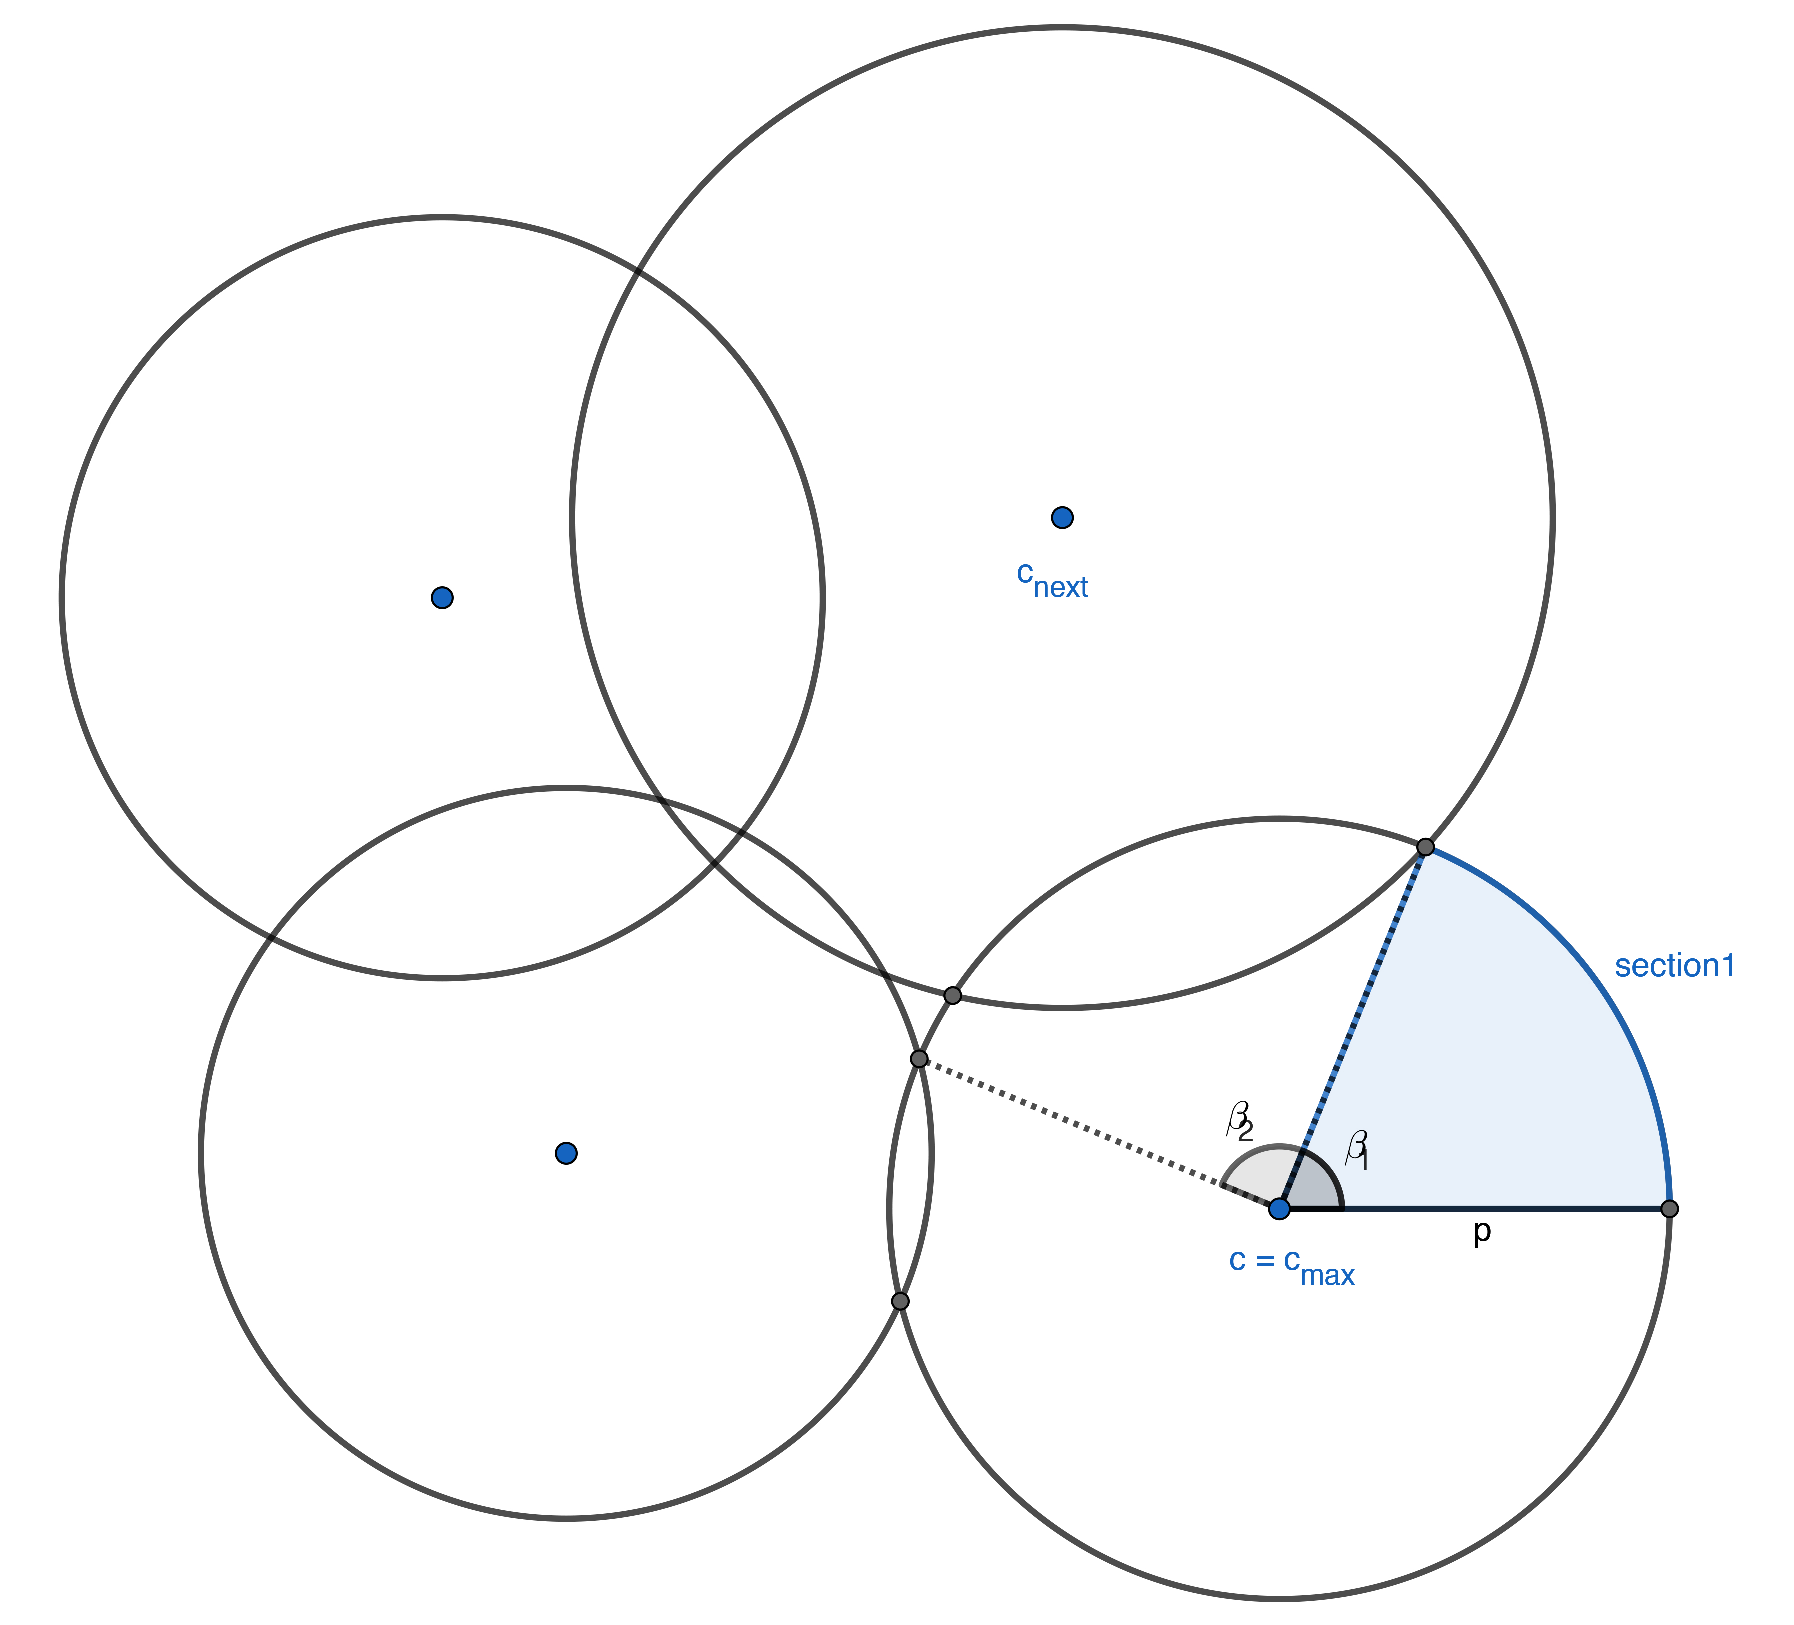
\includegraphics[width=1.0\textwidth]{figures/contour/c1copy.pdf}
    \caption{Finding first contour section}\label{fig:contour1}
  \endminipage\hfill
  \minipage{0.32\textwidth}
    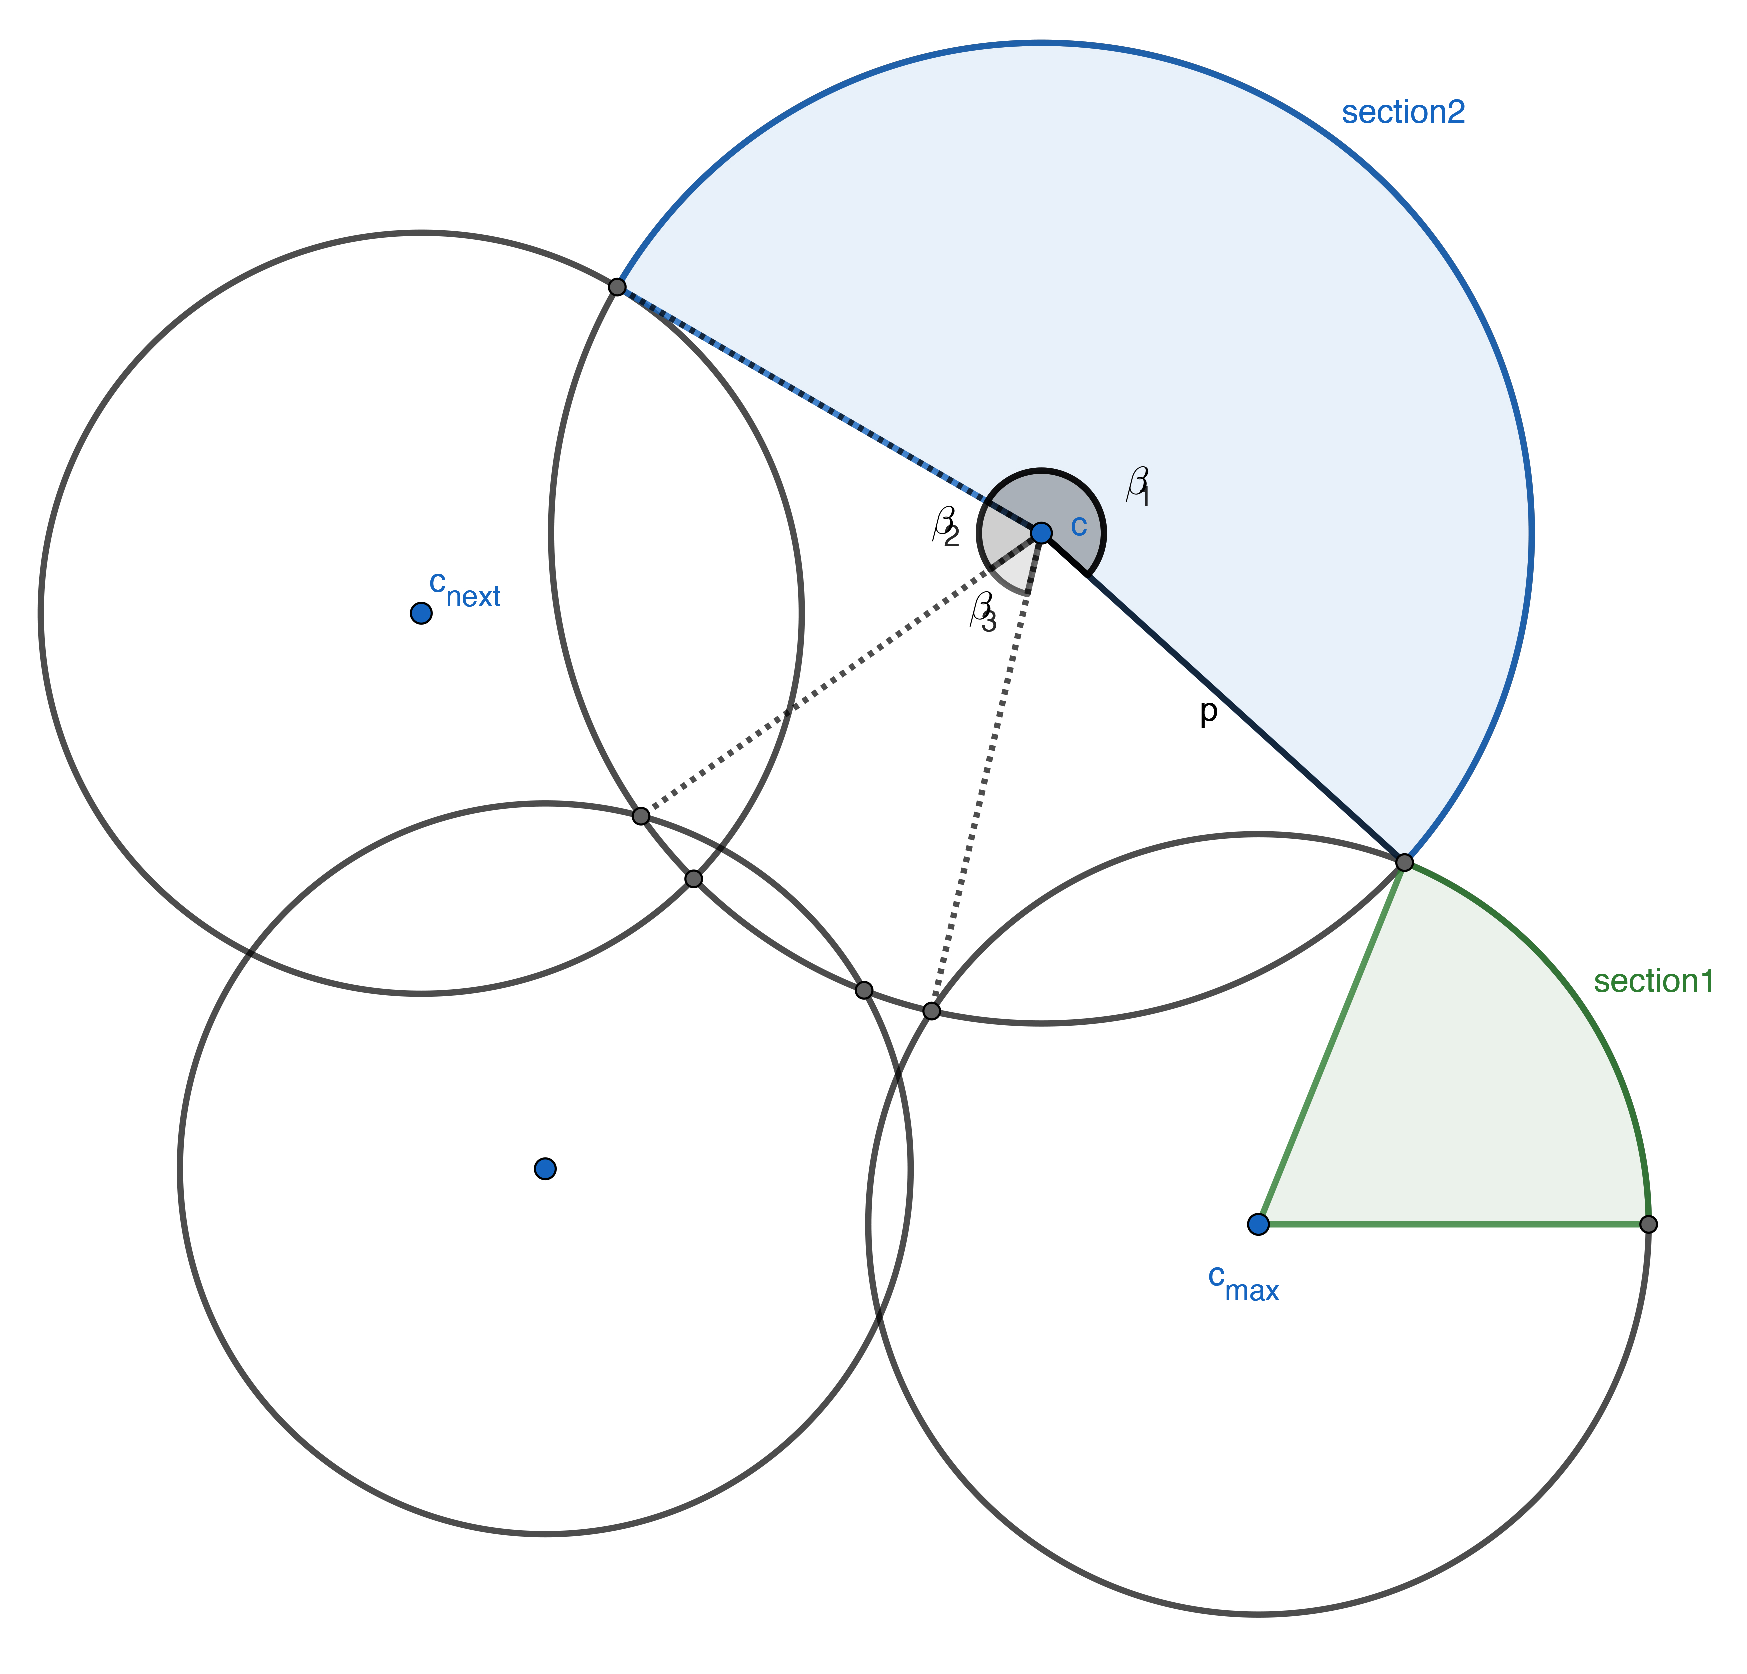
\includegraphics[width=1.0\textwidth]{figures/contour/c2copy.pdf}
    \caption{Finiding middle contour section}\label{fig:contour2}
  \endminipage\hfill
  \minipage{0.32\textwidth}%
    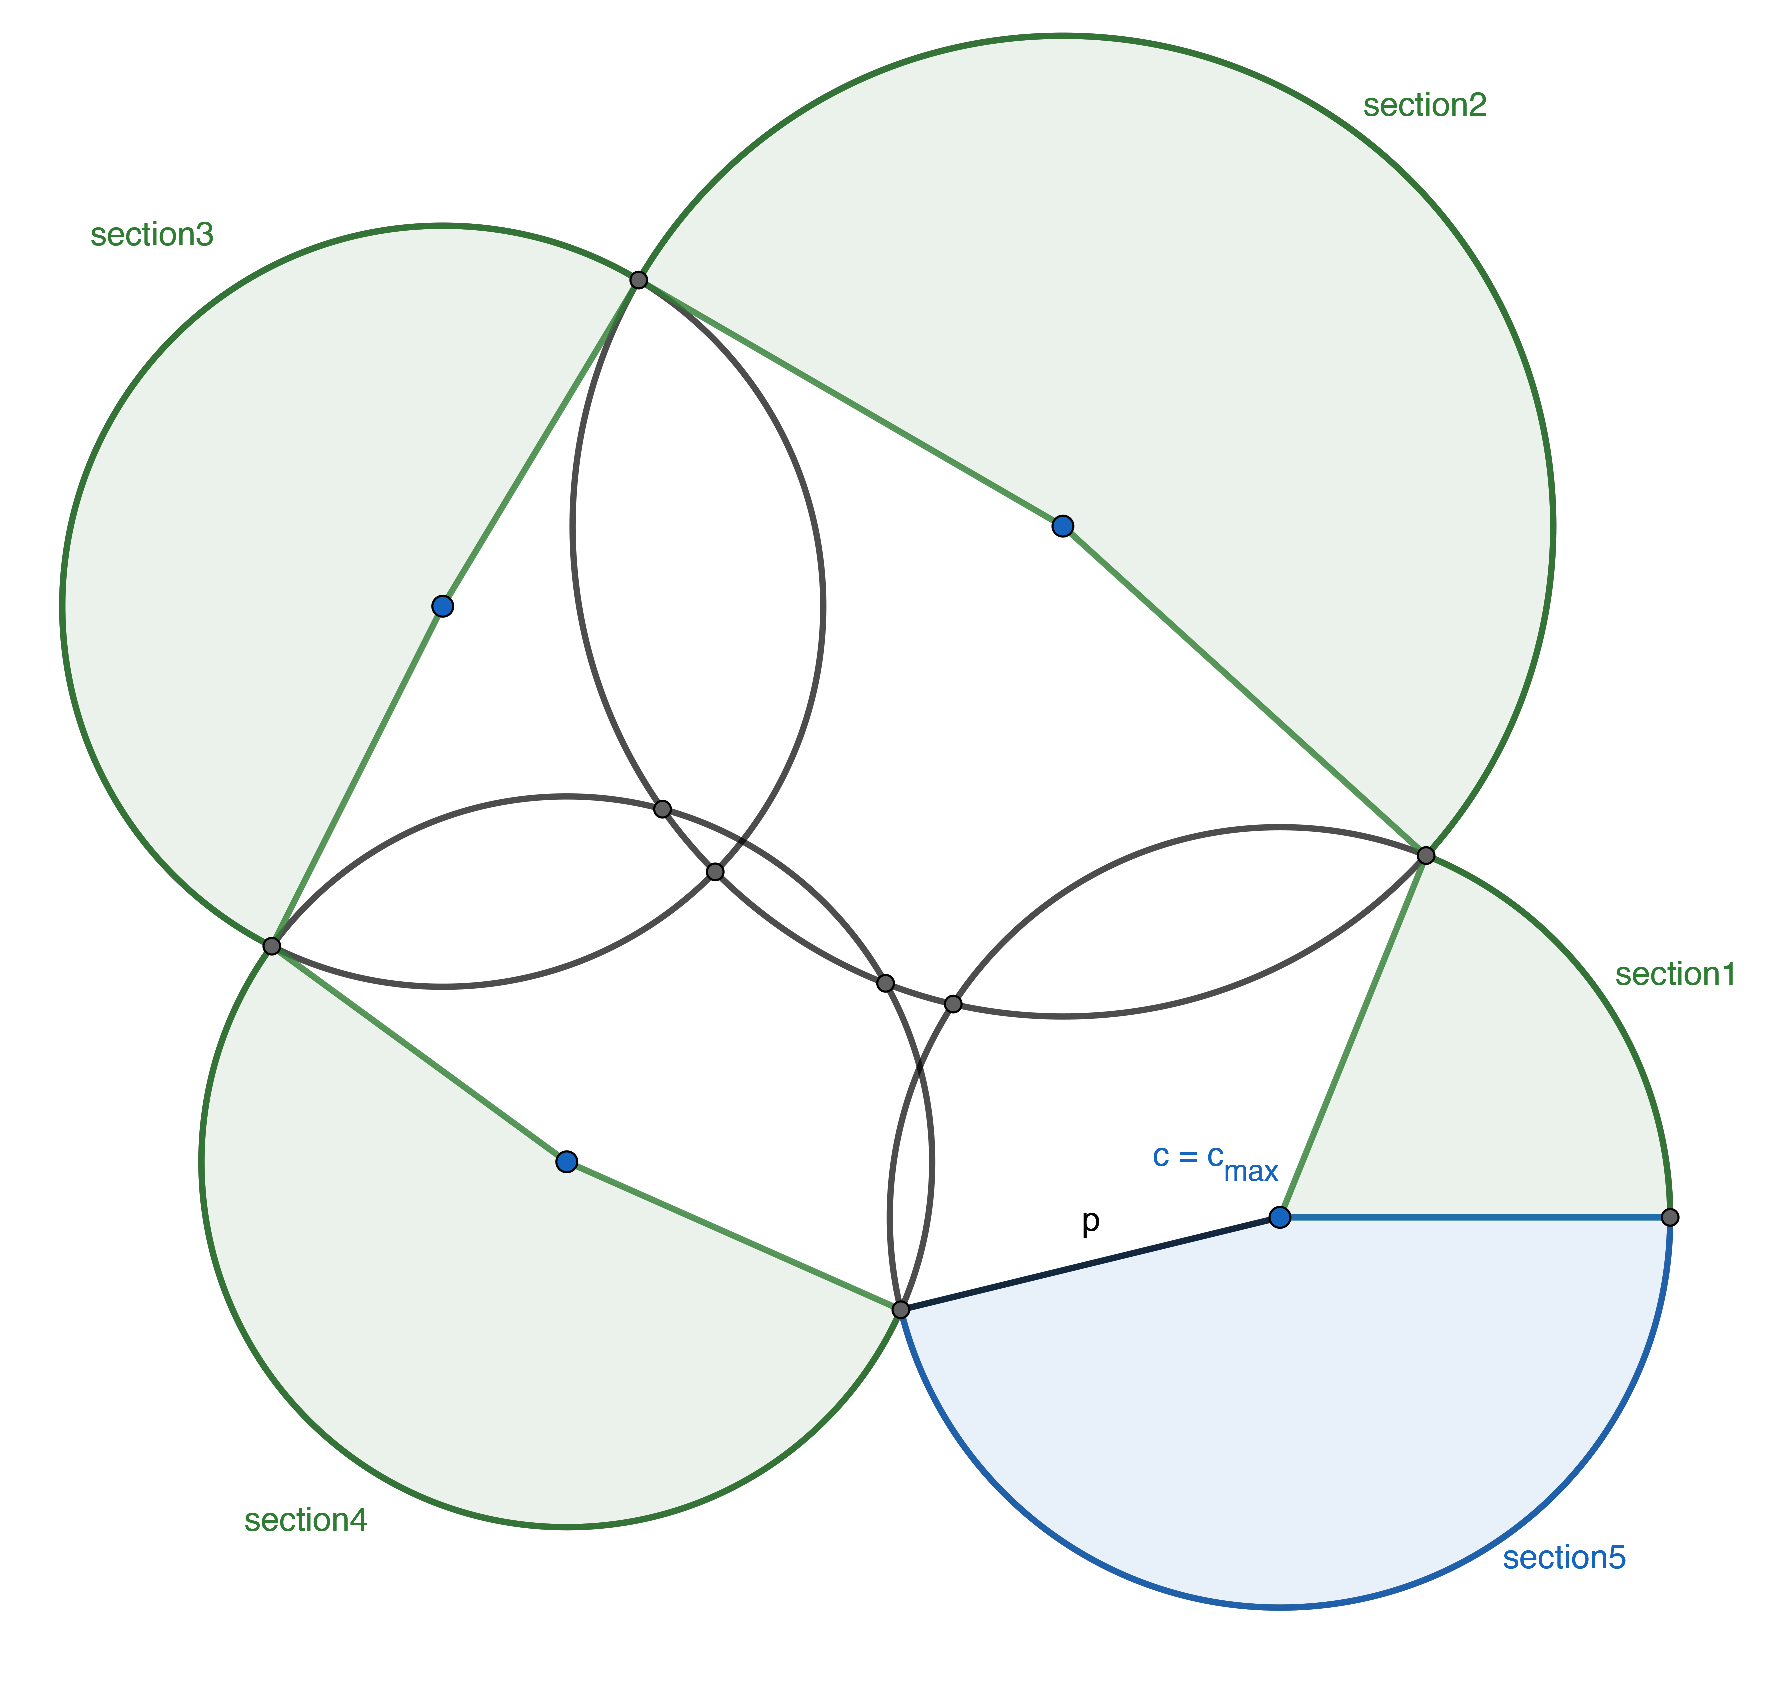
\includegraphics[width=1.0\textwidth]{figures/contour/c3copy.pdf}
    \caption{Finding the last contour section}\label{fig:contour3}
  \endminipage
\end{figure}



\chapter{Second Content Chapter}
\label{ch:SecondContent}

\dots

\section{First Section}
\label{sec:SecondContent:FirstSection}

\dots

\section{Second Section}
\label{sec:SecondContent:SecondSection}

\dots

Add additional content chapters if required by adding new .tex files in the
\code{sections/} directory and adding an appropriate 
\code{\textbackslash input} statement in \code{thesis.tex}. 
%% ---------------------
%% | / Example content |
%% ---------------------